\section{Evolutionary computing}

%Introduzione
\subsection{Introduzione}
Gli algoritmi evolutivi sono una classe di tecniche di ottimizzazione che imitano i principi dell'evoluzione biologica. Essi appartengono alla famiglia delle metaeuristiche. Il principio fondamentale degli algoritmi evolutivi è quello di applicare principi evolutivi come la mutazione e la selezione a popolazioni di soluzioni candidate al fine di trovare una soluzione (sufficientemente buona) per un dato problema di ottimizzazione.

\paragraph{Optimization problems}
Un \textit{problema di ottimizzazione} può essere descritto da una tripla $(\Omega,f,\prec)$ dove $\Omega$ è lo spazio di ricerca, $f$ è una funzione di valutazione della forma $f:\Omega \to \mathbb{R}$ e $\prec$ un preordine. L'insieme $H \subseteq \Omega$ tale che:
$$H = \{ x \in \Omega | \forall x' \in \Omega: f(x) \succeq f(x') \}$$
è definito l'insieme degli \textit{ottimi globali}. Dato un problema di questo genere la sua soluzione sta nel fornire un elemento che appartiene all'insieme $H$

Gli \textit{algoritmi evolutivi} rispondono a questo problema adottando una strategia innovativa. \uline{Tali algoritmi sono direttamente ispirati alla teoria della evoluzione biologica}

\paragraph{Principi fondamentali evoluzione biologica}
Gli algoritmi evolutivi sono tra le metaeuristiche più antiche e popolari. Sono essenzialmente basati sulla teoria dell'evoluzione biologica di Charles Darwin proposta nel libro “\textit{Le origini delle specie}”, che esprime la diversità e complessità di tutte le forme di vita. Il principio alla base dell’evoluzione biologica consiste in:
\begin{enumerate}
    \item Tratti vantaggiosi che sono risultato di mutazioni casuali tendono ad essere favoriti dalla selezione naturale
    \item Gli individui che mostrano questi tratti vantaggiosi hanno migliori opportunità di procreare e moltiplicarsi
\end{enumerate}
È importante comprendere che un tratto non è benefico o dannoso di per sé, ma solo in relazione all'ambiente\footnote{Un pigmento della pelle scuro può essere utile in Africa per difendersi dai raggi ultravioletti ma altrove può condurre una carenza di vitamina D; oppure l’anemia (la ridotta capacità di trasportare ossigeno nel sangue) che però protegge dalla malaria, ed è quindi un vantaggio in alcuni regioni.}

\paragraph{Elementi di un algoritmo evolutivo}
Un algoritmo evolutivo richiede i seguenti elementi
\begin{enumerate}
    \item una \textbf{\textit{codifica}} per i candidati di soluzione. Poiché vogliamo evolvere una popolazione di candidati di soluzione, abbiamo bisogno di un modo per rappresentarli come cromosomi, cioè dobbiamo codificarli, essenzialmente come sequenze di oggetti computazionali (bit, caratteri, numeri, ecc.).
    \item Un metodo per creare una \textbf{\textit{popolazione iniziale}}. Poiché i cromosomi sono semplici sequenze di oggetti computazionali, una popolazione iniziale viene comunemente creata generando semplicemente sequenze casuali
    \item Una \textbf{\textit{funzione di fitness}}, indica le probabilità di sopravvivere e riprodursi, dovuti alla capacità di adattarsi all’ambiente. Spesso è la funzione da ottimizzare
    \item \textbf{\textit{Metodi di selezione}} rispetto ai valori di fitness. Si scelgono così gli individui che dovranno procreare nella successiva generazione
    \item \textbf{\textit{Operatori genetici}} che modificano i cromosomi. Utilizzati negli algoritmi genetici per generare nuove soluzioni candidate attraverso la manipolazione dei geni o delle caratteristiche delle soluzioni esistenti. I nuovi tratti possono essere creati da diversi processi, i più utilizzati sono:
    \begin{itemize}
        \item \textit{Mutazione}, introduce una piccola perturbazione casuale in una soluzione candidata. Avviene modificando casualmente uno o più geni della soluzione.
        \item \textit{Crossover}, è un operatore che simula il processo di riproduzione sessuale. Nelle forme di vita con riproduzione sessuata vengono presi elementi dai DNA dei genitori per comporre il DNA della prole. Durante le prime fasi della moltiplicazione cellulare il DNA viene ripetutamente ricombinato (per questo è anche chiamato ricombinazione) creando così nuovi tratti.
    \end{itemize}

    Nella maggior parte dei casi le mutazioni sono sfavorevoli o addirittura letali, ma c’è una piccola probabilità che siano invece vantaggiose, ovvero che aiutino la sopravvivenza. Ogni nuovo individuo è “testato” subito dall’ambiente che lo circonda, se il nuovo tratto è sfavorevole l’individuo non sopravvive e il tratto così sparisce dalla popolazione.
    
    \item \textit{Vari parametri}, come dimensione della popolazione, probabilità di mutazione. Ad esempio, la dimensione della popolazione da evolvere, la frazione di individui scelti da ogni popolazione per produrre discendenti, la probabilità che si verifichi una mutazione in un individuo, ecc
    \item \textbf{\textit{Condizione di terminazione}}, numero di generazioni, approssimazioni all'ottimo
\end{enumerate}

Per ogni problema di ottimizzazione occorre separare lo spazio dei \textit{fenotipi} $\Omega$, come l'individuo appare, ciò che interagisce con l’ambiente e a cui viene applicata la funzione di fitness, da quello dei \textit{genotipi} $\Gamma$, come l'individuo è rappresentato dalla codifica scelta e su cui agiscono gli operatori genetici. La funzione di fitness sarà definita sui fenotipi, gli operatori genetici agiranno sui genotipi. Per valutare i cambiamenti nel genotipo sarà necessario provvedere una funzione di decodifica $dec: \Gamma \to \Omega$.

\paragraph{Individuo}
E' un organismo vivente in biologia, e corrisponde nel nostro caso ad un candidato alla soluzione del problema. Ogni \textit{individuo} $A$ è rappresentato da un tupla $(A.G, A.S, A.F)$ contenente il genotipo ($A.G \in \Gamma$), informazioni e parametri addizionali $A.S \in Z$ e la valutazione dello stesso rispetto alla funzione di fitness $A.F = f(dec(A.G))$.

\paragraph{Gene}
E' una parte del cromosoma, è l’unità fondamentale che si va ad ereditare e definisce un tratto, come il colore degli occhi.

\paragraph{Allele}
Un allele è la possibile forma di un gene in biologia, se un gene rappresenta il colore degli occhi, ha degli alleli che codificano il colore blu, o marrone, o verde ecc. C’è un solo allele per ciascun gene.

\paragraph{Popolazione}
Una popolazione è un insieme di individui della stessa specie (di norma).

\paragraph{Generazione}
Una generazione si riferisce alla popolazione in un momento del tempo specifico.

\paragraph{Operatore di mutazione}
E' definito come una mappa
$$Mut^{\xi} : \Gamma \times Z \to \Gamma \times Z$$
dove $\xi$ è un numero randomicamente generato.

\paragraph{Operatore di ricombinazione}
Avente $r \geq 2$ genitori e $s \geq 1$ figli è definito come una mappa
$$Rek^\xi : (\Gamma \times Z)^r \to (\Gamma \times Z)^s$$
dove $\xi$ è un numero randomicamente generato

\paragraph{Operatore di selezione}
Ci permette di scegliere grazie ai valori di fitness tra una popolazione di $r$ individui un numero $s$ di individui che continueranno la specie. Sia $P = \{A_1, \dots, A_r \} $ la popolazione di individui allora l'operatore di selezione avrà la forma:
$$Sel^\xi : (\Gamma \times Z \times \mathbb{R})^r \to (\Gamma \times Z \times \mathbb{R})^s$$
$$A_{i \quad 1 \leq i \leq r} \mapsto A_{IS^\xi (c_1,\dots,c_r)_k \quad 1 \leq k \leq s } $$
dove la selezione ha la forma
$$IS^\xi : \mathbb{R}^r \to \{ 1, \dots, r \}^s$$

\paragraph{Definizione formale di algoritmo evolutivo}
Un algoritmo evolutivo su un problema di ottimizzazione $P$ è una tupla $$(\Gamma, dec, Mut, Rek, IS_{genitori}, IS_{ambiente}, \mu, \lambda)$$
Dove $dec$ è la decoding function, $IS_{genitori}$ è la selection function applicata ai genitori, $IS_{ambiente}$ è la selection function che identifica altri elementi nella popolazione la cui selezione deriva da fattori ambientali $\mu$ descrive il numero degli individui della generazione precedente e $\lambda$ descrive il numero di figli da generare per la generazione successiva.

Si può fare una distinzione all'interno degli algoritmi evolutivi
\begin{itemize}
    \item \textit{Algoritmi genetici}
    \item \textit{Algoritmi evolutivi}
\end{itemize}


%Meta-euristiche
\subsection{Meta-euristiche}
Le meta-euristiche sono tecniche computazionali piuttosto generali che vengono tipicamente utilizzate per risolvere problemi di ottimizzazione numerica e combinatoria in modo approssimato in più iterazioni. Le meta-euristiche vengono generalmente definite come una sequenza astratta di operazioni su determinati oggetti e possono essere applicate a problemi essenzialmente arbitrari. Tuttavia, gli oggetti su cui operano e i passaggi da effettuare devono essere adattati al problema specifico.

Le metaeuristiche vengono di solito applicate a problemi per i quali non è noto un algoritmo di soluzione efficiente, cioè problemi per i quali tutti gli algoritmi conosciuti hanno una complessità temporale (asintotica) esponenziale rispetto alla dimensione del problema. Nella pratica, tali problemi possono raramente essere risolti in modo esatto, a causa delle elevate richieste di tempo di calcolo e/o di potenza di calcolo. Di conseguenza, è necessario accettare soluzioni approssimate, e questo è ciò che le meta-euristiche possono fornire

\paragraph{Local search method}
E' un tipo di meta-euristica che cerca di trovare il massimo globale di una funzione di ottimizzazione attraverso l'ispezione di punti vicini a quelli scelti in fase di inizializzazione. Questo metodo si basa sull'idea che la funzione non abbia salti significativi tra i punti vicini. A differenza di altri algoritmi evolutivi, questo utilizza solo un singolo individuo e si concentra sulla mutazione piuttosto che sulla ricombinazione. Durante ogni iterazione, l'algoritmo decide se continuare a modificare l'individuo attuale o crearne uno nuovo per evitare minimi o massimi locali. Il gradient ascent/descent viene utilizzato per identificare il punto di massimo/minimo, con l'ampiezza dei passi che deve essere bilanciata per evitare oscillazioni o convergenza lenta. 

Per evitare di rimanere bloccati in minimi o massimi locali, l'algoritmo viene eseguito su diversi punti. 

Tutti questi metodi sono talvolta chiamati metodi di ricerca locale, perché compiono solo piccoli passi nello spazio di ricerca e quindi effettuano una ricerca locale di soluzioni migliori

\paragraph{Hill climbing}
Il termine Hill Climbing indica la capacità dell'algoritmo di scalare i nodi verso quelli con valori maggiori. Lo spazio di ricerca dell'algoritmo è limitato ai soli nodi vicino a quello corrente. Il rischio è quello di incappare in un massimo locale.

Se la funzione $f$ non è differenziabile, la discesa o l'ascesa del gradiente non è un'opzione. Tuttavia, possiamo cercare di determinare una direzione in cui $f$ aumenta valutando punti casuali nelle vicinanze del punto corrente. Il risultato è noto come \textit{hill climbing}

\paragraph{Simulated annealing}
Il \textit{simulated annealing} è una generalizzazione di questo approccio che prevede l'accettazione di soluzioni peggiori in base alla loro "qualità". Si basa sul principio che “la transizione da un massimo locale più basso ad uno più alto è più probabile della transizione in direzione opposta”. Le soluzioni migliori sono sempre tenute in considerazione, mentre le soluzioni peggiori sono anch’esse considerate con una certa probabilità e un parametro \textit{temperatura} che decresce nel tempo: soluzioni peggiori sono più accettabili all’inizio dell’esplorazione dello spazio invece che alla fine, per consentire una convergenza.

\paragraph{Tabu search}
La Tabu Search è un algoritmo di ricerca locale che tiene conto della storia delle generazioni precedenti durante la creazione di una nuova soluzione. L'obiettivo è evitare di ritornare su soluzioni già esplorate in passato e di superare i possibili ottimi locali. Durante l'esecuzione dell'algoritmo, viene mantenuta una lista Tabu, che funziona come una coda FIFO, in cui vengono registrati i candidati già esplorati. Questi candidati sono \textit{tabù} e non vengono considerati nelle fasi successive della ricerca, in modo da evitare cicli ripetitivi

L'obiettivo principale della Tabu Search è quello di esplorare lo spazio delle soluzioni in modo più efficace, superando i possibili ottimi locali e cercando di raggiungere la migliore soluzione globale

%Elementi di algoritmi evolutivi
\subsection{Elementi di algoritmi evolutivi}
Gli algoritmi evolutivi non sono procedure fisse, ma contengono diversi elementi che devono essere adattati al problema di ottimizzazione da risolvere

\subsubsection{Codifica}
\uline{Il modo in cui le soluzioni candidate al problema di ottimizzazione vengono codificate può avere un notevole impatto sulla facilità con cui un algoritmo evolutivo trova una soluzione buona}. In generale, è importante prestare attenzione all'interazione tra la codifica scelta e gli operatori genetici. Se la codifica riduce lo spazio di ricerca, ma si scopre essere difficile trovare operatori genetici che garantiscono che il risultato della loro applicazione sia in questo spazio di ricerca ridotto, potrebbe essere necessario gestire tali casi.

Non esiste una ricetta generale, il problema della codifica è specifico per ogni problema. Possiamo identificare le seguenti proprietà che una codifica dovrebbe avere
\begin{itemize}
    \item[I)] \textit{\textbf{Hamming Cliffs}}, rappresentare fenotipi simili con genotipi simili. Due genotipi sono ovviamente simili se differiscono di alcuni geni, perché servono poche mutazioni per passare da un genotipo all’altro. Possiamo definire la similarità dei genotipi con quanti operatori genetici servono per mutare da un genotipo all’altro.

    Gli Hamming cliffs si verificano quando due genotipi o sequenze di bit che rappresentano soluzioni simili a livello fenotipico (cioè soluzioni candidate simili) hanno una grande distanza di Hamming a livello genotipico, cioè differiscono per molti bit. In altre parole, gli Hamming cliffs si presentano quando due soluzioni simili richiedono molte mutazioni o modifiche dei bit per trasformare una sequenza nella sua controparte simile. 
    \item[II)] \textit{\textbf{Epistasis}}, la funzione di fitness deve restituire valori simili per candidati simili. In biologia l’epistasi è il fenomeno in cui l’allele di un gene sopprime gli effetti di tutti i possibili alleli di un altro gene. Negli algoritmi evolutivi descrive l’interazione tra due geni di un cromosoma: quanto cambia la fitness di una soluzione se si cambia un suo gene.
    \item[III)] \textit{\textbf{Closedness of the Search Space}}, lo spazio $\Omega$ deve essere chiuso rispetto agli operatori genetici. Tutte le soluzioni possibili sono rappresentate, nessuna soluzione non possibile è rappresentata. Se non è chiuso ci possono essere soluzioni che non sono codificabili ed interpretate 
\end{itemize}

\subsubsection{Fitness and selection}
Alla base della selezione c’è il principio che gli individui migliori hanno migliori probabilità di procreare e contribuire alla creazione delle nuove generazioni. Questo processo di selezione deve essere bilanciato attraverso l'uso della cosiddetta \textbf{\textit{selective pressure}}\footnote{La selective pressure, o pressione selettiva, è un parametro chiave negli algoritmi genetici che influenza la probabilità di selezione degli individui durante il processo di riproduzione e creazione delle nuove generazioni}, che può essere bassa per favorire l'esplorazione dello spazio di ricerca o alta per sfruttare gli individui migliori vicini all'ottimo. 
\begin{itemize}
    \item Un’alta selective pressure indica che anche piccole differenze nella fitness tra individui danno probabilità molto diverse di procreare: sfruttiamo gli individui migliori, perché solo quelli con alta fitness hanno buone possibilità di riprodursi
    \item Una bassa selective pressure indica che le probabilità di riprodursi degli individui dipendono poco dalle differenze nei valori di fitness: favoriamo l’esplorazione dello spazio di ricerca, anche individui in regioni con basso fitness hanno buone possibilità di riprodursi
\end{itemize}
La strategia migliore per scegliere la selective pressure giusta è time-dependent: nelle prime generazioni tenerla bassa, e alzarla mano a mano fino alle ultime generazioni. Possiamo usare metriche come:
\begin{itemize}
    \item \textit{Selection intensity}, valutare la differenza tra i valori di fitness prima e dopo la selezione
    \item \textit{Time to takeover/tempo di convergenza},  indica il numero di generazioni necessarie affinché la popolazione converga verso una soluzione ottima o di alta qualità. Questo valore riflette la velocità con cui l'algoritmo genetico è in grado di individuare e sfruttare le soluzioni migliori presenti nello spazio di ricerca
\end{itemize}
$$f_{rel}(A_i) = \frac{A_i.F}{\sum_{j=1}^{|P|} A_j.F}$$
La probabilità per un individuo di essere selezionato per la riproduzione sarà proporzionale al suo valore di fitness relativo. Alcuni svantaggi
\begin{itemize}
    \item La computazione del valore di fitness relativo è costosa e difficilmente parallelizzabile
    \item Scomparsa delle biodiversità, perchè gli individui con un alto valore di fitness potrebbero dominare la selezione
    \item Molto veloce a trovare ottimi locali, ma pessima esplorazione dello spazio
\end{itemize}

\subsubsection{Selezione}
Varie strategie disponibili in letteratura per operare la selezione degli individui che costituiranno il pool genetico per la successiva generazione
\begin{itemize}
    \item \textit{Roulette-wheel selection}, il funzionamento della roulette-wheel selection è simile a una ruota della roulette in cui ogni individuo ha un settore proporzionale alla sua probabilità di selezione. La somma delle probabilità di tutti gli individui corrisponde a un intero giro della ruota. Per selezionare un individuo, viene generato casualmente un numero tra $0$ e la somma delle probabilità e viene eseguita una scansione dei settori della ruota fino a quando il numero casuale è compreso all'interno di un settore. L'individuo corrispondente a quel settore viene selezionato.

    Nella roulette-wheel selection, gli individui con un rank o un valore di fitness più alto avranno settori più ampi sulla ruota, aumentando così la loro probabilità di essere selezionati
    \item \textit{Rank-based selection}, si ordinano gli individui in ordine di fitness decrescente. A seconda della posizione si assegna ad ogni individuo un rank e con esso si definisce la probabilità di essere selezionati. Si procede ad una selezione del tipo roulette-wheel. Lo svantaggio sta che occorre ordinare gli individui, complessità $O(n \log n)$ dove $n$ è il numero degli individui
    \item \textit{Tournament selection}, si estraggono $k$ individui casualmente dalla popo- lazione. Tramite confronti individuali, basandosi su rank o valore di fitness si decide il migliore, il quale riceverà la possibilità di riprodursi nella prossima generazione. Si riesce così ad evitare il problema della dominanza\footnote{Il problema della dominanza si riferisce alla situazione in cui un individuo con un rank o un valore di fitness molto alto domina gli altri individui, impedendo loro di essere selezionati o influenzando significativamente la diversità genetica della popolazione} perché ogni scontro individuale offre una possibilità per gli individui meno dominanti di emergere come vincitori e avere la possibilità di riprodursi
    \item \textit{Elitismo}, in tutti i casi precedenti non ci sono garanzie che i migliori passino da una generazione alla successiva. Con l’etilismo un numero selezionato di individui migliori passa direttamente alla generazione successiva per preservare l’elite. Il vantaggio è che la convergenza viene ottenuta rapidamente. Lo svantaggio è che c’è il rischio di rimanere bloccati in ottimi locali, poiché gli individui di élite vengono mantenuti senza subire modifiche, potrebbero non essere in grado di esplorare nuove regioni dello spazio di ricerca che potrebbero contenere soluzioni migliori.
    \item \textit{Crowding}, individui delle generazioni successive rimpiazzano individui simili a loro. La densità locale in $\Gamma$ non può crescere in modo indefinito, questo permette una migliore esplorazione dello spazio. Per implementare il crowding, è necessario definire una metrica di distanza o similarità tra gli individui, comunemente si utilizza la distanza euclidea o la distanza di Hamming, a seconda della codifica utilizzata. Gli individui più simili tra loro saranno quelli che avranno una distanza più piccola. Durante il processo evolutivo, quando si selezionano gli individui per la riproduzione, vengono scelti quelli che hanno una bassa similarità con gli individui già presenti nella popolazione. In altre parole, si preferiscono gli individui che sono "diversi" dagli altri.
\end{itemize}

\subsubsection{Operatori genetici}
Fungono da strumenti per esplorare lo spazio di ricerca. Tali operatori servono principalmente a produrre una soluzione candidata che sia (molto) simile al genitore. Se le soluzioni candidate sono codificate come stringhe di bit (ovvero, i cromosomi sono composti da zeri e uni), la mutazione bit (nota anche come inversione di bit) è comunemente scelta. Consiste nel capovolgere casualmente gli alleli selezionati, cioè trasformare un $1$ in $0$ e viceversa. 

Gli operatori genetici sono comunemente categorizzati in base al numero di genitori in \textit{mutation (one parent) operator}; \textit{crossover (two-parent)}; \textit{multi-parent operator}. Le ultime due categorie, cioè con più di un genitore, sono talvolta chiamate genericamente operatori di ricombinazione.

\paragraph{Mutation/One parent operator}
Nella prima classe possiamo trovare l’operatore di mutazione. Introduce biodiversità e favorisce l’esplorazione dello spazio di ricerca. Esistono vari metodi per operare una mutazione
\begin{enumerate}
    \item \textit{Standard mutation}, sostituisce l'allele corrente di un gene scelto casualmente con un altro allele scelto casualmente   
    \begin{figure}[h]
        \centering
        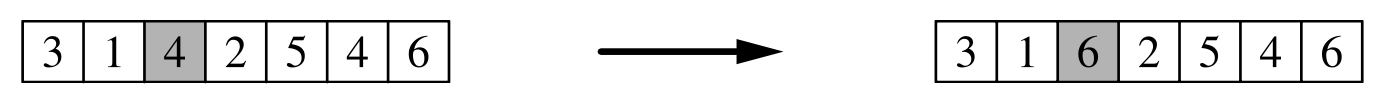
\includegraphics[scale=0.35]{images/standard-mutation.png}
        \caption{Esempio di standard mutation: un allele di un gene viene sostituito da un altro allele}
    \end{figure}
    \item \textit{Pair swap}(trasposizione), swap della posizione di due geni
    \begin{figure}[h]
        \centering
        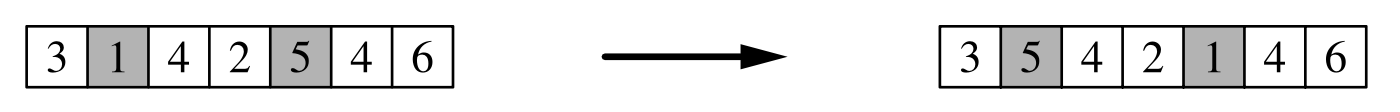
\includegraphics[scale=0.35]{images/pair-swap-mutation.png}
        \caption{Esempio di trasposizione: due geni scambiano i loro alleli in un cromosoma}
    \end{figure}
    \item \textit{Shift}, shifta a destra o sinistra un gruppo di geni
    \item \textit{Inversion}, invertire l'ordine degli alleli
    \item \textit{Arbitrary permutation}, permutazione arbitraria di un gruppo di geni
    \begin{figure}[h]
        \centering
        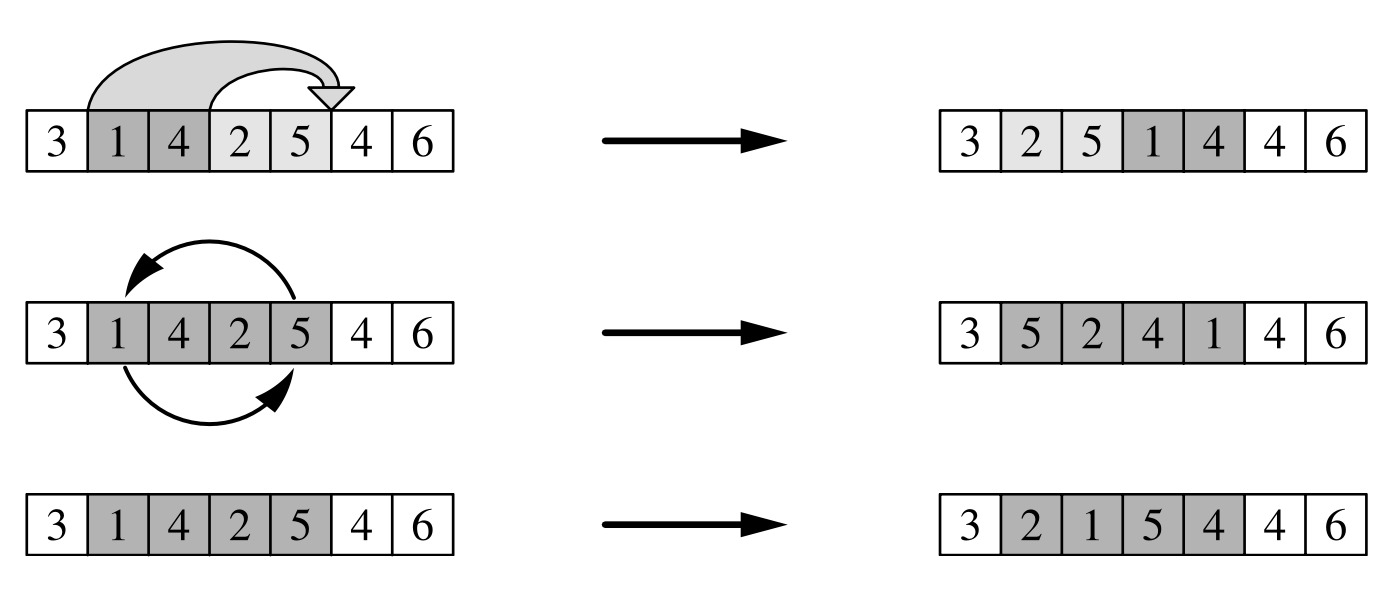
\includegraphics[scale=0.35]{images/shift-inversion-aribitrary.png}
        \caption{Operatori di mutation su sottosequenze: shift, inversion e arbitrary permutation}
    \end{figure}
\end{enumerate}
\paragraph{Crossover/Two parent operator}
Vari modi per ricombinare
\begin{enumerate}
    \item \textit{One-point crossover}, viene scelto casualmente un cut point e le sequenze di geni su un lato di questo punto vengono scambiate tra i due cromosomi 
    \begin{figure}[h]
        \centering
        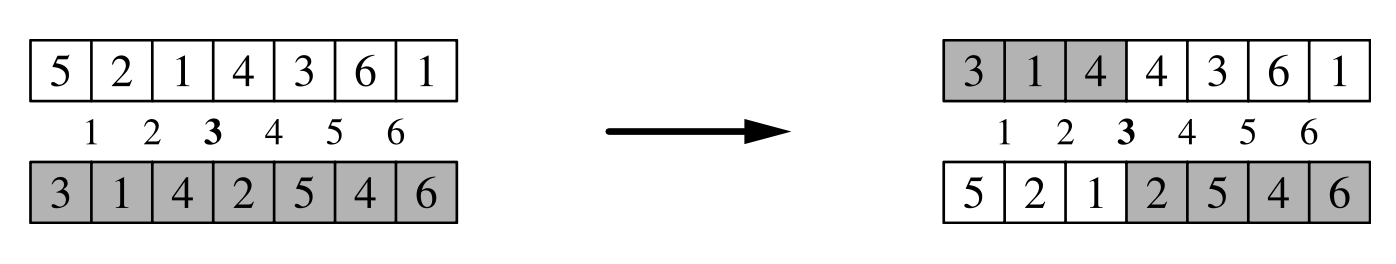
\includegraphics[scale=0.35]{images/one-point-crossover.png}
        \caption{Esempio di one-point crossover}
    \end{figure}
    \item \textit{Two-point crossover}, è un'estensione diretta del one-point crossover. In questo caso, vengono scelti due cut point casuali e la sezione compresa tra i due punti  viene scambiata tra i cromosomi.
    \begin{figure}[h]
        \centering
        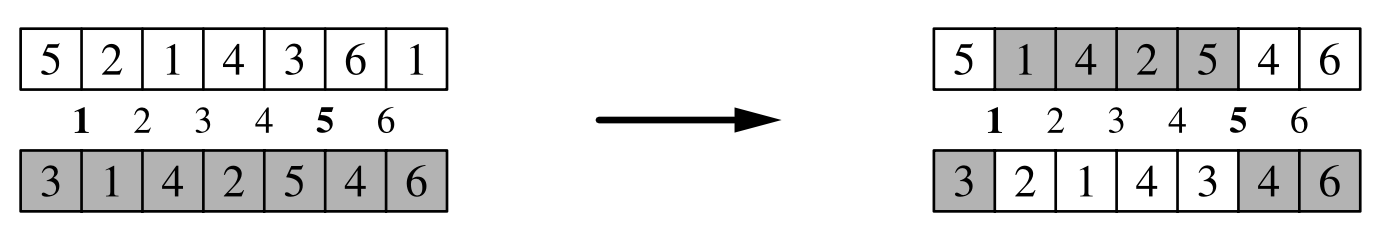
\includegraphics[scale=0.35]{images/two-point-crossover.png}
        \caption{Esempio di two-point crossover}
    \end{figure}
    \item \textit{N-point crossover}, un generalizzazione dei precedenti. Si scambiano le aree incluse nei punti selezionati casualmente
    \item \textit{Uniform crossover}, per ogni gene si determina se scambiarlo o meno a seconda di un certo parametro di probabilità $p_x$
    \item \textit{Shuffle crossover}, mescola casualmente i geni prima di applicare un operatore arbitrario a due genitori e quindi ripristina l'ordine originale dei geni. Prima una permutazione randomica, poi one-point crossover, poi unmixing
    \item \textit{Uniform order-based crossover}, operatore genetico utilizzato per combinare i geni di due genitori in modo flessibile e casuale. Utilizza una maschera di crossover per selezionare casualmente le posizioni dei geni da entrambi i genitori, creando discendenti con maggiore variabilità e potenzialmente esplorando una più ampia gamma di soluzioni nell'ottimizzazione e nella ricerca.
    \item \textit{Edge-recombination crossover}, il cromosoma è rappresentato come un grafo. Ogni gene è un vertice che ha archi verso i suoi vicini. Gli archi dei due grafi vengono mischiati. Si preserva l’informazione relativa alla vicinanza (permutazione).
\end{enumerate}

\paragraph{Multiple parent operator}
Il \textit{diagonal crossover} è un operatore di ricombinazione che può essere applicato a tre o più genitori ed è una generalizzazione del one-point crossover. Dati $k$ genitori, si scelgono $k-1$ punti per il crossover e si procede shiftando diagonalmente le sequenze rispetto ai punti scelti. Il crossover diagonale è considerato un metodo molto efficace per esplorare lo spazio di ricerca, specialmente quando si hanno un gran numero di genitori (circa $10$-$15$).
\begin{figure}[h]
    \centering
    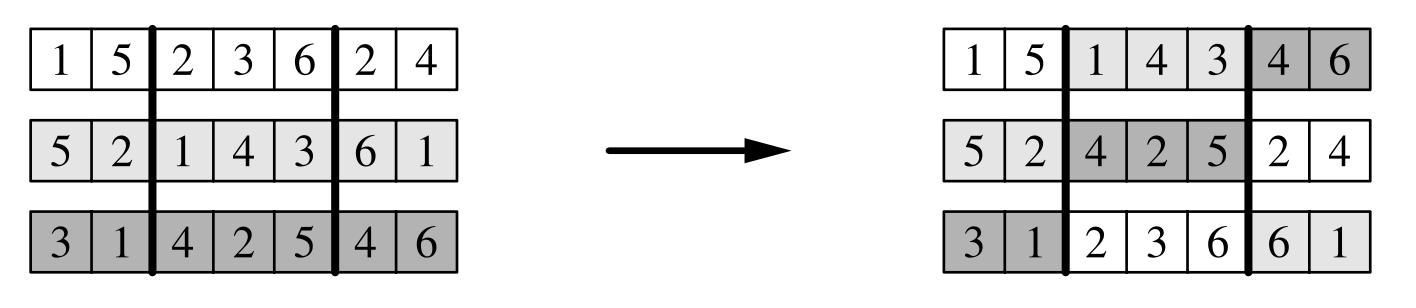
\includegraphics[scale=0.35]{images/diagonal-crossover.png}
    \caption{Esempio di diagonal crossover}
\end{figure}

\paragraph{Caratteristiche operatori crossover}
Gli operatori di ricombinazione sono spesso categorizzati in base a determinate proprietà
\begin{itemize}
    \item \textit{Positional bias}, quando \uline{la probabilità che due geni vengano ereditati assieme dallo stesso genitore} dipende dalla posizione (relativa) dei due geni nel cromosoma. Deve essere evitato perché può rendere la disposizione dei geni cruciale per la riuscita dell’algoritmo.

    Un esempio semplice di un operatore di ricombinazione che mostra un bias posizionale è il one-point crossover: la probabilità che due geni vengano ereditati congiuntamente è più alta quando i geni sono più vicini nel cromosoma. Ciò avviene perché i geni vicini hanno solo pochi cut points possibili tra di loro. Solo se uno di questi punti viene scelto, i geni vengono separati. Poiché tutti i cut points hanno la stessa probabilità, la probabilità che due geni siano ereditati congiuntamente è inversamente proporzionale al numero di punti di taglio tra di loro e quindi alla loro distanza nel cromosoma. Un caso estremo è rappresentato dal primo e l'ultimo gene di un cromosoma, che non possono mai essere ereditati congiuntamente mediante one-point crossover poiché qualsiasi punto di taglio li separa. Due geni vicini in un cromosoma vengono separati dal one-point crossover con una probabilità di $\frac{1}{L - 1}$, dove $L$ è la lunghezza del cromosoma.
    \item \textit{Distributional bias}, un operatore di ricombinazione presenta un bias distributivo se la probabilità che un certo numero di geni venga scambiato tra i cromosomi genitori non è la stessa per tutti i possibili numeri di geni. Il bias distributivo di solito è meno critico (più tollerabile) rispetto al bias posizionale. Un esempio semplice di un operatore di ricombinazione che presenta un bias distributivo è il crossover uniforme. 
\end{itemize}
Un esempio di operatore di crossover che non presenta né un bias posizionale né un bias distributivo è il crossover shuffle basato sul one-point crossover.

\paragraph{Migliorare le performance} Due strategie per migliorare le performance
\begin{itemize}
    \item \textit{Interpolating recombination}, avviene attraverso una combinazione lineare dei geni dei genitori. Ogni gene del discendente è calcolato come una media ponderata dei geni corrispondenti dei genitori. Ad esempio, se abbiamo due genitori $A$ e $B$ con i geni $[1, 3, 5]$ e $[2, 4, 6]$, rispettivamente, e utilizziamo un peso di $0.5$ per entrambi i genitori, il discendente $C$ avrà i geni $[\frac{1+2}{2}, \frac{3+4}{2}, \frac{5+6}{2}] = [1.5, 3.5, 5.5]$. Questo processo di combinazione lineare permette di creare discendenti con caratteristiche medie dei genitori originali.
    \item \textit{Extrapolating recombination} oltre alla media ponderata dei geni dei genitori, viene introdotto un fattore di estensione che permette di generare nuovi valori al di là dei limiti dei genitori. Ad esempio, se abbiamo due genitori $A$ e $B$ con i geni $[1, 3, 5]$ e $[2, 4, 6]$, rispettivamente, e utilizziamo un fattore di estensione di $1.5$, il discendente $C$ avrà i geni $[1.5\cdot(1-2), 1.5\cdot(3-4), 1.5\cdot(5-6)] = [-1.5, -1.5, -1.5]$. Questo processo permette di esplorare nuove regioni dello spazio delle soluzioni durante la ricerca e l'ottimizzazione, potenzialmente portando a soluzioni più diverse e innovative.
\end{itemize}

\subsubsection{Swarm and population based optimization}

\paragraph{Swarm intelligence}
La swarn intelligence è un'area di ricerca nell'intelligenza artificiale che si concentra sullo studio del comportamento collettivo di popolazioni di agenti semplici. I sistemi di swarm intelligence sono spesso ispirati al comportamento di alcune specie animali, in particolare insetti sociali come formiche e api, nonché animali che vivono e cercano cibo in gruppi come pesci, uccelli e lupi. Questi animali, cooperando tra loro, sono spesso in grado di risolvere problemi piuttosto complessi. Ad esempio, possono trovare i percorsi più brevi per fonti di cibo, costruire nidi, cacciare prede. Esistono varie tipologie di euristiche di questo genere
\begin{itemize}
    \item \textit{Particle swarm optimization}, ispirato al pattern biologico della ricerca del cibo in uccelli e pesci. Gli individui aggregano informazioni, creando un insieme di conoscenze comuni, al fine di presentare una sola soluzione. Ogni individuo è un candidato ad essere la soluzione
    \item \textit{Ant colony optimization}, ispirato al pattern biologico delle formiche che cercano una strada che le conduca al cibo. Gli individui scambiano informazioni modificando l’ambiente, in modo che gli altri possano seguire (o meno) le loro tracce. Ogni individuo è un candidato ad essere la soluzione
\end{itemize}

\paragraph{Population based incremental learning}
In questa tecnica di ottimizzazione, gli individui sono generati casualmente utilizzando una distribuzione di probabilità. Non è necessario conservare esplicitamente ogni singolo individuo nella memoria, ma è sufficiente mantenere le statistiche della popolazione, come ad esempio la media e la deviazione standard delle soluzioni.

Per la \textit{ricombinazione}, viene utilizzato l'operatore \textit{uniform crossover}. La selezione degli individui si basa sul miglioramento delle statistiche della popolazione, cioè si scelgono gli individui che portano a una media migliore o a una deviazione standard più piccola.

La \textit{mutazione}, invece, prevede solo un semplice \textit{bit-flip}, ovvero un cambiamento casuale di un singolo bit nel genotipo. Una caratteristica distintiva di questa tecnica è che il tasso di apprendimento, ovvero il parametro che regola la velocità di movimento degli individui nello spazio delle soluzioni, cambia nel tempo e si riduce con il numero di iterazioni.

\subsubsection{Fondamenti teorici}
\uline{Per verificare la validità degli algoritmi evolutivi, è necessario considerare gli \textit{schemata}, che sono cromosomi binari parzialmente specificati che codificano un comportamento particolare}. Questi schemata possono essere utilizzati per studiare l'evoluzione nel tempo del numero di cromosomi che condividono lo stesso schema.

L'obiettivo è quello di fornire una stima statistica di come gli algoritmi evolutivi esplorano lo spazio di ricerca. In questo modo, è possibile valutare l'efficacia degli algoritmi e capire come essi si comportano nella ricerca di soluzioni ottimali.

\begin{definizione}
    Uno schema $h$ è una stringa di caratteri di lunghezza $L$ sull'alfabeto ${0, 1 \∗}$, cioè $h \in {0, 1, \∗}L$ . Il carattere $\∗$ è chiamato carattere jolly o don't care symbol
\end{definizione}

\begin{definizione}
    Un cromosoma $c$ si dice che \textit{condivide} lo schema $h$ (in simboli, $c \triangleleft h$) se e solo se, escluse le posizioni in $h$ aventi il simbolo $*$, $h$ coincide con $c$.
\end{definizione}

A titolo di esempio sia $h$ uno schema di lunghezza $L = 10$ e $c1$, $c2$ due diversi cromosomi di questa lunghezza, che appaiono così:
$$h = \ast01110$$
$$c1 = 1100111100$$ 
$$c2 = 1111111111$$

Chiaramente, il cromosoma $c1$ corrisponde allo schema $h$, cioè $c1 \triangleleft h$, perché $c1$ differisce da $h$ solo nelle posizioni in cui $h$ è $\ast$. D'altra parte, il cromosoma $c2$ non corrisponde a $h$, cioè $c2 \ntriangleleft h$ , perché $c2$ contiene $1$ nelle posizioni in cui $h$ è $0$ (posizioni $3$ e $9$).

In un algoritmo genetico, la fitness rappresenta la capacità di un cromosoma di risolvere un determinato problema o di adattarsi a un ambiente specifico. Quando si utilizzano schemi specifici per analizzare la popolazione di cromosomi, la fitness viene calcolata solo per quei cromosomi che condividono lo schema in questione. Ad esempio, se lo schema specifico è rappresentato da una sequenza di bit "1101", allora solo i cromosomi che contengono questa sequenza esatta di bit verranno considerati nella valutazione della fitness. L'ordine di uno schema è importante perché indica quanti bit all'interno dello schema devono essere mantenuti costanti per preservare l'efficacia dello schema durante la mutazione.

Per calcolare l'influenza dell'operatore di mutazione su uno schema specifico, occorre valutare la probabilità che lo schema venga preservato dopo la mutazione. Ciò significa che, dopo che un cromosoma è stato sottoposto a mutazione, occorre valutare se lo schema specifico è ancora presente e, in caso contrario, determinare se la mutazione ha portato a un miglioramento o a una riduzione della fitness complessiva del cromosoma

%Strategie evolutive
\subsection{Strategie evolutive}
In una strategia evolutiva, \uline{consideriamo l'intero processo evolutivo, non solo l'ottimizzazione dei singoli individui}. Prendiamo in considerazione parametri come riproduzione, mortalità, e la lunghezza media della vita degli individui, che dipendono dalle scelte che facciamo riguardo agli operatori genetici. Rappresentiamo il problema di ottimizzazione come una funzione $f: \mathbb{R}^n \to \mathbb{R}$ che vogliamo minimizzare, e utilizziamo array di reali come rappresentazione dei cromosomi. Utilizziamo solo l'operatore di mutazione per spostare i cromosomi all'interno dello spazio di ricerca aggiungendo un vettore randomico $r$ ottenuto da una distribuzione normale. 

\paragraph{Selection}
La selezione nelle strategie evolutive segue un rigoroso principio di élite: solo i migliori individui passano alla generazione successiva. Nonostante il principio di élite sia fisso, esistono due diverse forme di selezione, che si distinguono dal fatto che vengono considerati solo i discendenti o se i genitori e i discendenti insieme sono presi in considerazione nel processo di selezione. Sia $\mu$ il numero di individui nella generazione dei genitori e $\lambda$ il numero di individui discendenti creati per mutazione:
\begin{itemize}
    \item \textit{Plus-strategy}, i genitori e i figli vengono raggruppati per il processo di selezione, ossia la selezione viene effettuata su $\mu + \lambda$ individui
    \item \textit{Comma-strategy}, la selezione considera solo gli individui discendenti
\end{itemize}


%Programmazione genetica
\subsection{Programmazione genetica}
Con la genetic programming (GP) si cerca di evolvere espressioni simboliche o addirittura programmi informatici con determinate proprietà.

Finora abbiamo considerato solo cromosomi che erano array di lunghezza fissa, ad esempio array di bit per gli algoritmi genetici o array di numeri reali per le strategie evolutive. Per la programmazione genetica, abbandoniamo la restrizione a una lunghezza fissa e permettiamo cromosomi di lunghezza variabile.

La base formale è una grammatica che descrive il linguaggio dei programmi genetici. Seguendo l'approccio standard dei linguaggi formali, definiamo due insiemi, ovvero l'insieme $\mathcal{F}$ di simboli di funzione e operatori e l'insieme $\mathcal{T}$ di costanti e variabili. $\mathcal{F}$ e $\mathcal{T}$ dovrebbero essere limitati in dimensione al fine di ridurre lo spazio di ricerca a una dimensione fattibile, ma "abbastanza ricchi" per consentire una soluzione al problema.

A titolo di esempio, supponiamo di voler apprendere una funzione booleana che mappa $n$ input binari in output binari associati. In questo caso, i seguenti insiemi di simboli sono una scelta naturale:
$$\mathcal{F} = \{\text{and}, \text{or}, \text{not}, \text{if} \dots then \dots else \dots\}$$
$$\mathcal{T} = \{x1, \dots, xn, 1, 0\}\;\; \text{o}\;\; T = \{x1, \dots, xn, \text{vero}, \text{falso}\}$$

Una proprietà desiderabile di $\mathcal{F}$ è che tutte le funzioni in esso siano complete nel dominio, ovvero dovrebbero accettare qualsiasi valore di input possibile. Semplici esempi di funzioni che non sono complete nel dominio sono la divisione, che provoca un errore se il divisore è zero, o il logaritmo, che di solito accetta solo argomenti positivi.

Un'altra proprietà importante è la completezza degli insiemi di funzioni $\mathcal{F}$ e $\mathcal{T}$ rispetto alle funzioni che possono rappresentare. La programmazione genetica può risolvere efficacemente un dato problema solo se $\mathcal{F}$ e $\mathcal{T}$ sono sufficienti per trovare un programma appropriato. Ad esempio, nella logica proposizionale booleana, $\mathcal{F} = \{\land, \lnot\}$ e $\mathcal{F} = \{\rightarrow, \lnot\}$ sono insiemi completi di operatori, perché qualsiasi funzione booleana con qualsiasi numero di argomenti può essere rappresentata da opportune combinazioni degli operatori in questi insiemi. Tuttavia, $\mathcal{F} = \{\land\}$ non è un insieme completo, perché non è possibile rappresentare nemmeno la semplice negazione di un argomento. Trovare il più piccolo insieme completo di operatori per un dato insieme di funzioni da rappresentare è (di solito) NP-hard. Di conseguenza, $\mathcal{F}$ di solito contiene più funzioni di quanto effettivamente necessario.

I programmi vengono rappresentati come alberi sintattici, dove i nodi interni rappresentano le operazioni e le foglie rappresentano le variabili o le costanti. Tuttavia, per risolvere un problema con successo, l'insieme di operazioni e simboli terminali deve essere \textit{completo} e \textit{sufficiente}

\paragraph{Parsing tree}
È conveniente rappresentare un'espressione simbolica mediante il cosiddetto albero di parsing. Gli alberi di parsing sono comunemente utilizzati, ad esempio, nei compilatori, soprattutto per le espressioni aritmetiche.

\paragraph{Inizializzazione}
Creare una popolazione iniziale è un po' più complesso nella programmazione genetica rispetto agli algoritmi evolutivi, perché non possiamo semplicemente creare sequenze casuali di simboli di funzione, costanti, variabili e parentesi. Data la complessità che esibiscono queste strutture, nel processo di creazione, bisogna considerare alcuni parametri quali l’\textit{altezza massima degli alberi} e il \textit{numero massimo di nodi}. Esistono vari sotto-algoritmi che si occupano dell’inizializzazione degli alberi sintattici:
\begin{itemize}
    \item \textit{Grow}, la probabilità di scegliere un nodo interno o uno terminale è distribuita in modo uniforme a qualsiasi livello di profondità. Questo permette di creare alberi sbilanciati
    \item \textit{Full}, i nodi terminali possono occorrere solo al livello dell’altezza massima dell’albero. Questo permette di creare alberi bilanciati
    \item \textit{Ramp-half-and-half}, i primi due metodi possono essere combinati creando metà della popolazione iniziale con il metodo grow e l'altra metà con il metodo full per avere più varianza nella forma esibita dagli alberi sintattici.  Questo metodo ha il vantaggio di garantire una buona diversità nella popolazione, con alberi di altezza e complessità diverse
\end{itemize}

\paragraph{Operatori genetici}
La popolazione iniziale della programmazione genetica (come in qualsiasi algoritmo evolutivo) di solito ha un valore di fitness molto basso, perché è altamente improbabile che una generazione casuale di parsing tree produca anche una soluzione vagamente adeguata. Per ottenere candidati di soluzioni migliori, vengono applicati gli operatori genetici. I tre più importanti sono: \textit{crossover}, consiste nello scambio di due sotto-espressioni (e quindi sotto-alberi nei parsing tree); \textit{mutation}; \textit{cloning} (duplicazione di un individuo)

È comune limitare la mutazione alla sostituzione di piccoli sotto-alberi (con un'altezza non superiore a tre o quattro), in modo da creare un individuo effettivamente simile. Una mutazione non limitata potrebbe sostituire l'intero albero di parsing, il che equivale a introdurre un individuo completamente nuovo.
Tuttavia, se la popolazione è sufficientemente ampia in modo che il "materiale genetico" presente garantisca una diversità adeguata, la mutazione spesso viene abbandonata e il crossover diventa l'unico operatore genetico\footnote{Questo è esattamente l'opposto delle strategie evolutive, in cui spesso si abbandona il crossover e la mutazione è l'unico operatore genetico}.

Il motivo è che il crossover, rispetto ad altri algoritmi evolutivi che lavorano con array di lunghezza fissa, è un operatore molto più potente. Ad esempio, se lo applichiamo a due individui identici, il semplice fatto che possano essere scelti diversi sotto-alberi crea la possibilità di ottenere due individui diversi.

\begin{figure}[h]
    \centering
    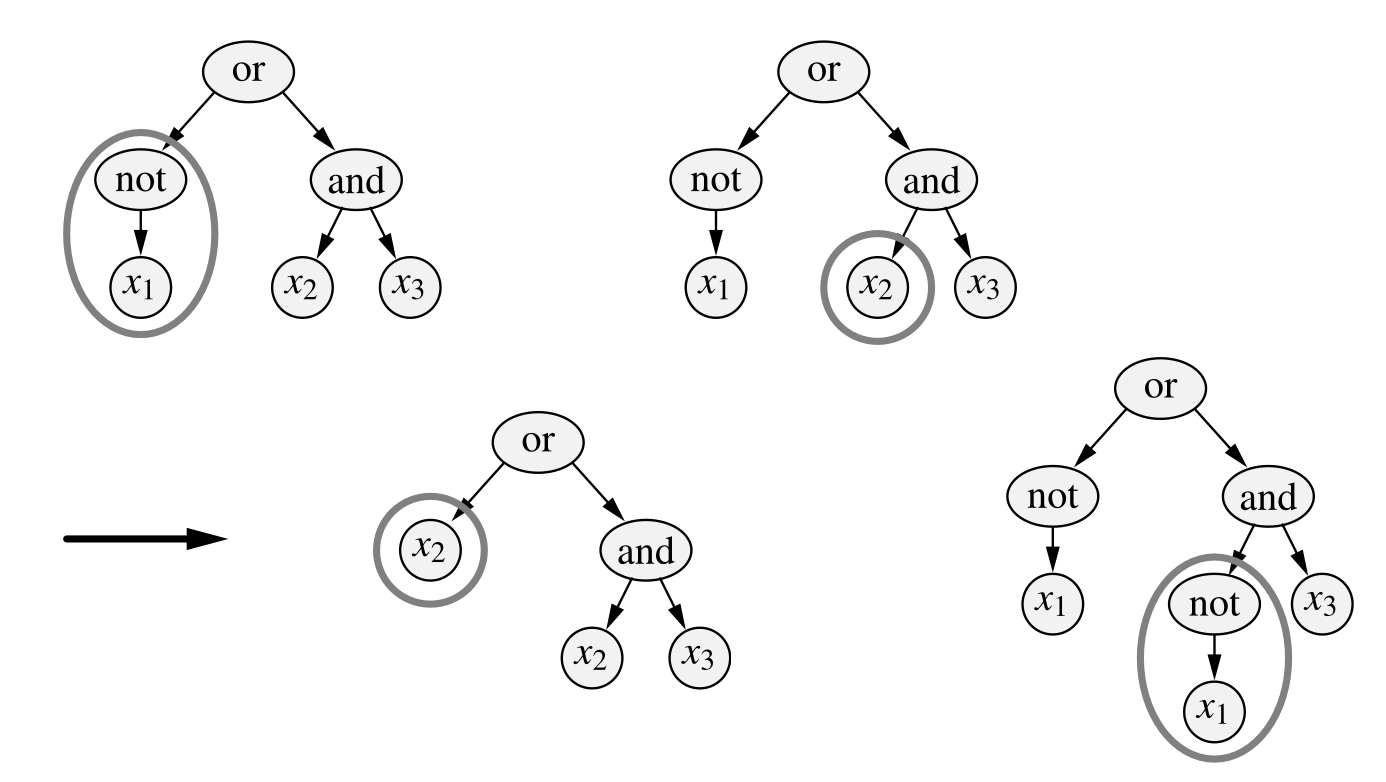
\includegraphics[scale=0.45]{images/gp-crossover.png}
    \caption{Vantaggio del crossover nella programmazione genetica rispetto agli operatori di crossover basati su array: applicato a due cromosomi identici, è possibile ottenere due figli diversi}
\end{figure}

\paragraph{Introni}
Durante il processo evolutivo gli individui tendono a sviluppare larghe porzioni di codice "inutile" ai fini della computazione. Un concetto simile viene dalla biologia: gli introni sono porzioni di DNA che non codificano alcuna informazione a livello del fenotipo (per questo vengono talvolta chiamati junk-DNA). 

Ad esempio, se vengono creati delle sotto-espressioni come $(\text{if}\;2 > 1\; \text{then}\; \dots\; \text{else}\; \dots)$, la parte else dell'istruzione condizionale è un introne, perché non può mai essere eseguita a meno che la condizione di test non venga modificata.

In generale, è consigliabile evitare la creazione di introni il più possibile, poiché gonfiano i cromosomi inutilmente, aumentano il tempo di elaborazione e rendono più difficile interpretare le soluzioni trovate.

Per evitare il verificarsi di questo fenomeno esistono alcune strategie:
\begin{itemize}
    \item \textit{Breeding recombination}, questo operatore crea molti figli dagli stessi due genitori applicando un operatore di crossover con parametri diversi. Solo il miglior figlio del gruppo entra nella generazione successiva
    \item \textit{Intelligent recombination}, sceglie intenzionalmente i punti di crossover
    \item \textit{Continuos slight changes} TODO $\dots$
\end{itemize}

%Multi-criteria optimization
\subsection{Multi-criteria optimization}
Nella vita quotidiana, ci troviamo spesso di fronte a situazioni che non possono essere descritte nella semplice forma dei problemi di ottimizzazione. In particolare, spesso ci troviamo di fronte al compito di selezionare tra un insieme di opzioni che soddisfano diversi criteri in modo differente. Molto spesso, questi criteri sono addirittura contrastanti, ossia cercare di migliorare uno fa sì che un altro criterio sia meno soddisfatto. Consideriamo, ad esempio, il compito di trovare un appartamento o di acquistare un bene di consumo. In generale, qualità e prezzo sono criteri in conflitto.

\paragraph{Weight combination of criteria}
Formalmente, l'ottimizzazione multi-criterio può essere descritta da $k$ funzioni obiettivo
$$f_i : \Omega \rightarrow \mathbb{R}, i = 1, \dots, k$$
Il nostro obiettivo è trovare un elemento dello spazio di ricerca per il quale tutte le funzioni restituiscono un valore il più alto possibile. L'approccio più semplice a questo problema è combinare tutte le k funzioni obiettivo in una singola funzione, riducendo così il problema a un problema di ottimizzazione standard. Ad esempio, possiamo calcolare una somma ponderata
$$f(s) = \sum^k_{i=1} w_i \cdot f_i(s)$$
dove i valori assoluti dei pesi specificano l'importanza relativa che attribuiamo ai diversi criteri. 

Sfortunatamente, un approccio basato sulla combinazione di diversi criteri in questo modo presenta gravi inconvenienti: oltre al fatto che potrebbe non essere facile scegliere pesi adeguati, perdiamo la possibilità di adattare le nostre preferenze relative in base alle proprietà delle soluzioni potenziali che otteniamo (cosa che sicuramente facciamo nei processi decisionali come la ricerca di un appartamento). Tuttavia, il problema è ancora più fondamentale: in generale, qui ci troviamo di fronte al problema di dover aggregare le preferenze.

\subsubsection{Pareto optimal solution}
Un approccio alternativo per combinare criteri multipli nell'ottimizzazione è cercare di trovare tutte o almeno molte soluzioni Pareto-ottimali.
\begin{definizione}
    Un elemento $s \in \Omega$ viene chiamato Pareto-ottimale rispetto alle funzioni obiettivo $f_i$ , $i = 1, \dots , k$ se non esiste alcun elemento $s\prime \in \Omega$ per il quale valgono le seguenti due proprietà:
    $$\forall i, 1\leq i \leq k: f_i(s\prime) \geq f_i(s)$$
    $$\exists i, 1 \leq i \leq k: f_i(s\prime) > f_i(s)$$
\end{definizione}
In modo intuitivo, l'ottimalità di Pareto significa che la soddisfazione di un qualsiasi criterio non può essere migliorata senza danneggiarne un altro.

Chiaramente, un vantaggio della ricerca di soluzioni Pareto-ottimali è che le funzioni obiettivo non devono essere combinate (e quindi non c'è bisogno di specificare pesi o una funzione di aggregazione). Inoltre, preserviamo la possibilità di adattare la nostra visione di quanto sia importante un criterio rispetto agli altri in base alle soluzioni che otteniamo. Tuttavia, lo svantaggio è che raramente esiste una sola soluzione Pareto-ottimale e quindi non esiste una soluzione univoca al problema di ottimizzazione

\begin{figure}[h]
    \centering
    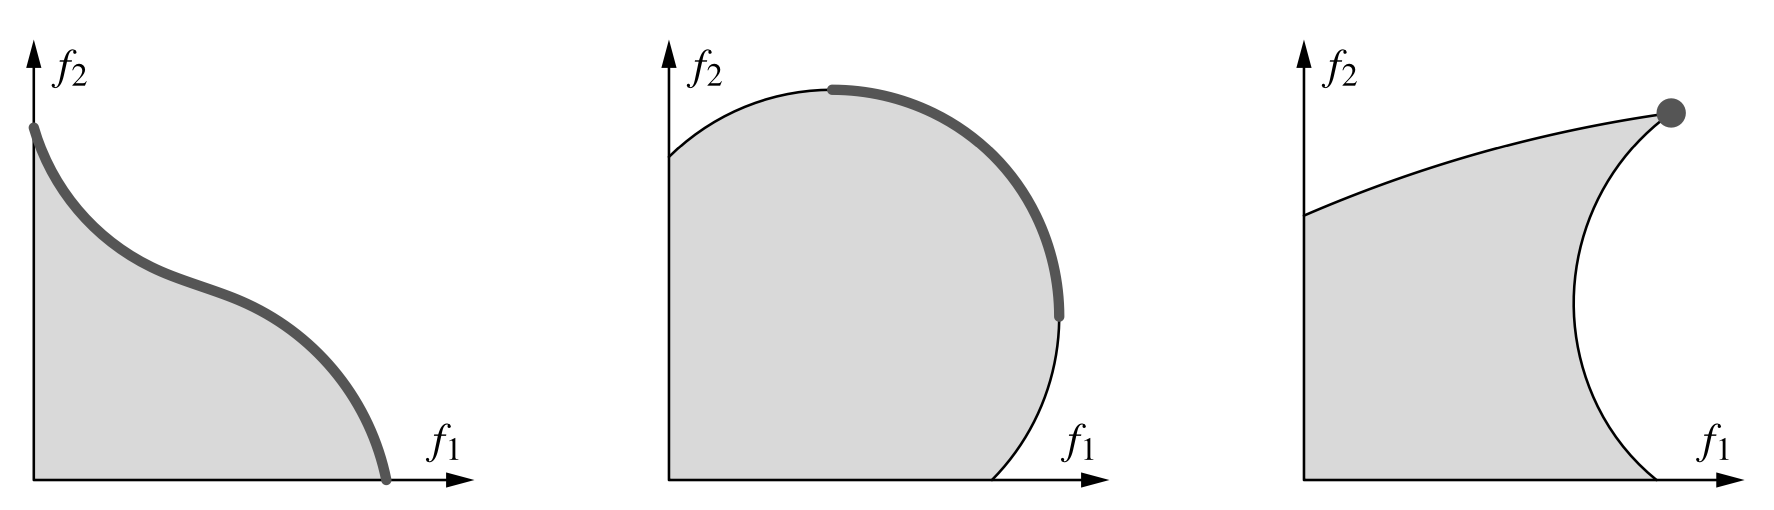
\includegraphics[scale=0.40]{images/pareto.png}
    \caption{Illustrazione delle soluzioni Pareto-ottimali, ovvero la cosiddetta frontiera di Pareto. Tutti i punti dello spazio di ricerca sono situati nell'area grigia (con le funzioni $f_1$ e $f_2$ che forniscono le coordinate). Le soluzioni Pareto-ottimali si trovano nella parte del confine disegnata in grigio scuro. Ad eccezione del diagramma a destra, ci sono molteplici soluzioni Pareto-ottimali}.
\end{figure}

\paragraph{Finding Pareto oprimal with Evolutionary Algorithms}
Fino ad ora abbiamo sempre supposto di avere una singola funzione da ottimizzare, gli algoritmi evolutivi possono essere applicati anche a problemi di ottimizzazione multi-criterio. In questo caso, \uline{l'obiettivo è trovare una selezione di candidati alla soluzione sulla frontiera di Pareto} o almeno vicino ad essa, che copra in modo sufficiente tale frontiera.

%Algoritmi evolutivi paralleli
\subsection{Algoritmi evolutivi paralleli}
Rispetto ad altre tecniche di ottimizzazione, gli algoritmi evolutivi sono noti per produrre risultati ottimali, ma con un costo computazionale elevato. Un modo per migliorare questa situazione è la parallelizzazione, ovvero la distribuzione delle operazioni necessarie su diversi processori. Si può parallelizzare:
\begin{itemize}
    \item La generazione iniziale è spesso facile da parallelizzare, poiché di solito i cromosomi vengono creati casualmente e in modo indipendente l'uno dall'altro
    \item Il calcolo del fitness degli individui
    \item La selezione se costituita da eventi indipendenti, come ad esempio tournament selection, diventa più complesso gestire etilismo
    \item L’applicazione degli operatori genetici
    \item Il controllo di raggiungimento del criterio di terminazione
\end{itemize}
Due architetture utilizzate sono: \textit{island model}; \textit{cellular evolution}

\paragraph{Island model and migration}
Facendo riferimento a una chiara analogia con la natura, ogni popolazione può essere vista come che abita un'isola, il che spiega il nome per questa architettura. Un modello di isole puro è equivalente all'esecuzione dello stesso algoritmo evolutivo più volte, che può essere fatto anche in modo seriale. Ogni isola avrà una popolazione, ed eseguirà il processo evolutivo. 

Un altro processo è noto come \textit{migration}. L'idea alla base di questo metodo è che il trasferimento di materiale genetico tra le isole migliori le proprietà esplorative delle popolazioni delle isole, senza necessità di ricombinazioni dirette tra cromosomi provenienti da isole diverse.
Esistono diverse modalità di migrazione tra le isole. Nel modello casuale, le coppie di isole vengono selezionate casualmente e scambiano alcuni dei loro individui. In questo caso, qualsiasi coppia di isole può teoricamente scambiarsi individui. Nel modello di rete, invece, le isole sono organizzate in una struttura di rete o grafo, e gli individui possono migrare solo tra isole connesse da un lato del grafo.

Sfruttando l'architettura a isole e la migrazione, è possibile ottenere una parallelizzazione efficace degli algoritmi evolutivi.

\paragraph{Cellular evolution}
Gli algoritmi evolutivi cellulari sono una forma di parallelizzazione chiamata anche \textit{isolation by distance}. Essi lavorano con un gran numero di processori (virtuali), ciascuno dei quali gestisce un singolo individuo, o solo un piccolo numero di individui. L'intero spazio di ricerca viene diviso in una griglia rettangolare.

Per la selezione, ogni processore valuta i cromosomi dei propri vicini e calcola il massimo tra di essi. Gli operatori genetici, come la mutazione o la ricombinazione, sono applicati solo tra i cromosomi dei vicini. In questo modo, ogni processore lavora indipendentemente, ma condivide informazioni con i suoi vicini per influenzare la selezione e l'evoluzione. La mutazione di un cromosoma è gestita da ogni singolo processore

\newpage